\section{Examples}

\subsection*{MCMC Univariate case}

In the given example, we are examining the application of Markov Chain Monte Carlo (MCMC) methods in a univariate context, where the target distribution of interest is the posterior distribution of a parameter \( \theta \) given observed data \( y \). The specific case involves a binomial likelihood where \( y \) conditional on \( \theta \) follows a binomial distribution, denoted by \( y | \theta \sim \text{bin}(n, \theta) \). The number of trials \( n \) is set to 100 and the number of successes \( y \) is 30.

Prior:
\[ f(\theta) = e^{-e^\theta} \]

Likelihood:
\[ L(\theta | y) = \binom{n}{y} \theta^y (1 - \theta)^{n-y} \propto \theta^y (1 - \theta)^{n-y} \]

Posterior:
\[ f(\theta | y) \propto f(\theta) \times L(\theta | y) \]
\[ f(\theta | y) \propto (e^{-e^\theta}) \theta^y (1 - \theta)^{n-y} \]

Proposal Distribution:
\[ \theta' | \theta \sim \text{Beta}(\alpha, \beta) \]
\[ \alpha = \theta, \quad \beta = 1 - \theta \]
\[ \Rightarrow \mathbb{E}[\theta' | \theta] = \frac{\alpha}{\alpha + \beta} = \theta \]

The prior distribution for \( \theta \) is chosen to be a function that favors neither extreme values of 0 or 1, indicated by \( f(\theta) = e^{-e^\theta} \), which is a function that could represent some non-standard beliefs about the parameter (like a preference for values away from 0 and 1). This prior is not a conventional choice like a beta distribution, which is commonly used as a conjugate prior for binomial likelihoods, but it demonstrates the flexibility of MCMC methods to accommodate various prior specifications.

The likelihood function \( L(\theta | y) \) follows from the binomial distribution and is given by the binomial coefficient times the probability of success raised to the number of successes and the probability of failure raised to the number of failures. The proportionality constant \( \alpha \) simplifies the expression, since the binomial coefficient does not depend on \( \theta \) and can be omitted in the calculation of the posterior.

The posterior distribution \( f(\theta | y) \) combines the prior and the likelihood via Bayes' theorem and is proportional to the product of these two functions. The posterior is what we aim to estimate using MCMC, as it gives the updated belief about \( \theta \) after observing \( y \).

The proposal distribution is specified to be a beta distribution with parameters \( \alpha \) and \( \beta \), which in the context of MCMC, is used to generate candidate values for \( \theta \) in the sampling process. The beta distribution is convenient for parameters like \( \theta \) that are constrained to the interval [0,1]. The choice of \( \alpha \) and \( \beta \) here suggests a symmetric proposal around the current value of \( \theta \) because the expected value \( E[\theta'] \) of the proposal distribution equals \( \theta \), ensuring that the proposal is centered at the current estimate.

% 
The Metropolis Hastings algorithm is implemented to estimate the posterior distribution of the parameter \( \theta \) based on observed binomial data. The algorithm generates a sequence of \( \theta \) values that approximate the distribution.

Starting with an initial guess \( \theta_{\text{init}} \), at each iteration, a new value \( \theta_{\text{prop}} \) is proposed by perturbing the current value with a normal distribution centered around \( \theta_{\text{current}} \) with a small standard deviation, reflecting a localized exploration of the parameter space.

The acceptance of \( \theta_{\text{prop}} \) is determined by the ratio \( \alpha \) of the posterior probabilities of the proposed and current \( \theta \) values. If \( \theta_{\text{prop}} \) falls outside the valid range \([0, 1]\), it is rejected, and \( \theta_{\text{current}} \) is retained. Otherwise, \( \theta_{\text{prop}} \) is accepted with a probability equal to \( \alpha \), ensuring that the chain gravitates towards areas of higher posterior probability.

We initiate chains from different starting values to inspect the robustness of the algorithm against initial conditions. The evolution of \( \theta \) over iterations is plotted, providing a visual representation of convergence behavior and the influence of initial values. This approach allows for an empirical investigation into the algorithm's mixing properties and convergence diagnostics, which are critical for assessing the reliability of MCMC methods in statistical inference.

\begin{figure}[htbp]
    \centering
    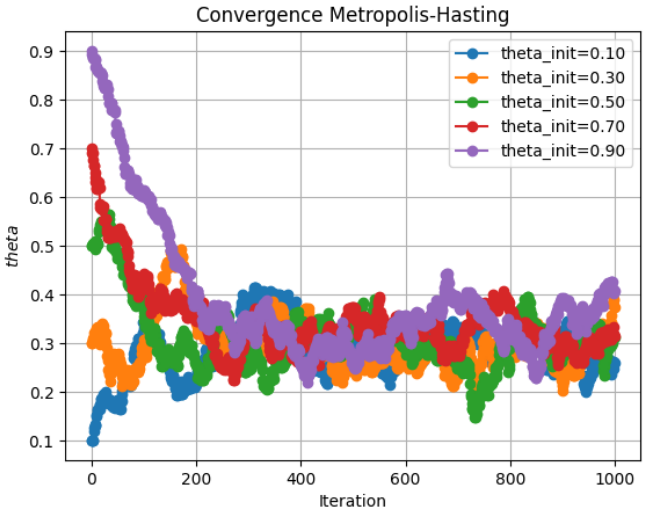
\includegraphics[width=\linewidth]{plots/output_univar.png}
    \caption{Convergence of markov chains from different initial values}
    \label{fig:my_label}
\end{figure}
    
\subsection*{MCMC Bivariate case}

In the current study, we extend the Markov Chain Monte Carlo (MCMC) framework to a bivariate case, addressing the scenario where two dependent probabilities are to be inferred. We denote the two observations as \( y = [y_1, y_2] \) and the corresponding parameters as \( \theta = [\theta_1, \theta_2] \). Each observation is assumed to be binomially distributed with \( y_1 \) trials and \( y_2 \) trials, leading to \( y_1 | \theta \sim \text{bin}(n_1, \theta_1) \) and \( y_2 | \theta \sim \text{bin}(n_2, \theta_2) \), respectively.

Given observations $y = [y_1, y_2]$ and parameters $\theta = [\theta_1, \theta_2]$, with $y_1 \sim \text{bin}(n_1, \theta_1)$ and $y_2 \sim \text{bin}(n_2, \theta_2)$, the Bayesian framework is applied to infer the posterior distributions of $\theta_1$ and $\theta_2$.


Prior :
\[f(\theta) = f(\theta_1) \times f(\theta_2)\]

likelihood :
\[
L(\theta_1, \theta_2 | y_1, y_2) = \binom{n_1}{y_1} \theta_1^{y_1} (1 - \theta_1)^{n_1-y_1} \binom{n_2}{y_2} \theta_2^{y_2} (1 - \theta_2)^{n_2-y_2}.
\]

Posterior :
\[
f(\theta | y) \propto f(\theta) \times L(\theta | y).
\]

Proposal distribution :
\[\theta' | \theta \sim \text{Multivariate Normal}, \text{mean} = \theta\]

The prior distribution for \( \theta \) is factored into the priors for \( \theta_1 \) and \( \theta_2 \), implying a belief in the independence of the two parameters a priori, \( f(\theta) = f(\theta_1) \times f(\theta_2) \).

The likelihood function \( L(\theta_1, \theta_2 | y_1, y_2) \) is constructed from the product of two binomial likelihoods, reflecting the probability of observing \( y_1 \) and \( y_2 \) given \( \theta_1 \) and \( \theta_2 \), respectively.

The posterior distribution \( f(\theta | y) \) is then proportional to the product of the prior distribution and the likelihood function. This proportional relationship is a result of Bayes' theorem, which updates our beliefs about the parameters \( \theta_1 \) and \( \theta_2 \) in light of the observed data \( y_1 \) and \( y_2 \).

To explore the posterior distribution, we propose new candidate values of \( \theta \) from a multivariate normal distribution with the mean equal to the current estimate of \( \theta \). This proposal mechanism accounts for the potential correlation between \( \theta_1 \) and \( \theta_2 \) in the posterior distribution, which is particularly relevant in bivariate or multivariate cases where parameters may not be independent.

The below plots show the convergence of markov chains for \( \theta_1 \) and \( \theta_2 \) for the meropolis hastings algorithm

In the above example the Metropolis Hastings algorithm is used to estimate the joint posterior distribution of \( \theta_1 \) and \( \theta_2 \).At each step, a candidate parameter vector \( \theta_{\text{prop}} \) is proposed by adding a bivariate normal perturbation to the current parameter estimate \( \theta_{\text{current}} \). This perturbation ensures a random walk that explores the parameter space around the current estimate.

The proposed parameters are accepted if they fall within the valid interval \([0, 1]\) for both dimensions, ensuring that the parameters remain within the bounds of probability values. The acceptance ratio \( \alpha \), computed as the ratio of the proposed and current probabilities (prior times likelihood), governs the transition between states. If a uniformly random number is less than \( \alpha \), the proposed parameters are accepted, updating \( \theta_{\text{current}} \) to \( \theta_{\text{prop}} \), and are otherwise discarded.

The result is a sequence of \( \theta \) values that represent samples from the joint posterior distribution, providing insights into the probable values of the parameters given the observed data and the specified model.

\begin{figure}[htbp]
    \centering
    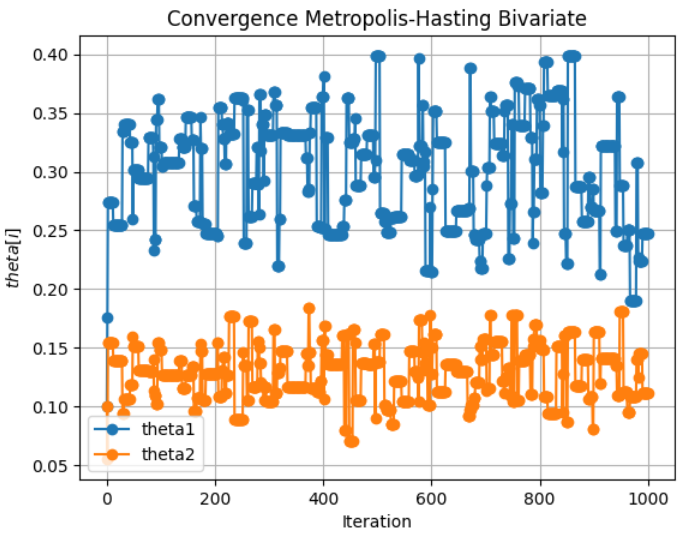
\includegraphics[width=\linewidth]{plots/output_bivar1.png}
    \caption{Convergence of markov chains for \( \theta_1 \) and \( \theta_2 \)}
    \label{fig:my_label}
\end{figure}
\begin{figure}[htbp]
    \centering
    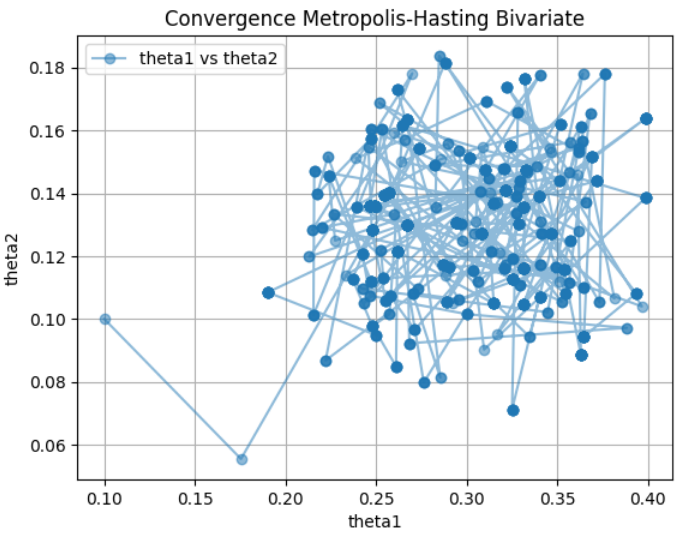
\includegraphics[width=\linewidth]{plots/output_bivar2.png}
    \caption{Convergence of metroplis chains for \( \theta_1 \) vs \( \theta_2 \)}
    \label{fig:my_label}
\end{figure}


\subsection*{MCMC Multivariate case}
In our research, we perform a Bayesian analysis using Markov Chain Monte Carlo (MCMC) on a dataset pertaining to vehicular stopping distances. The dataset comprises two variables: the speed of various vehicles and their corresponding stopping distances. We model the stopping distance as a linear function of speed, encapsulated by the equation \( y = ax + b + \varepsilon \), where \( \varepsilon \) is a normally distributed error term with mean zero and variance \( \sigma^2 \).

We define our parameter vector \( \theta = [a, b, \sigma] \) and express the likelihood of observing the data \( Y = [y_1, y_2, \ldots, y_n] \) given the speeds \( X = [x_1, x_2, \ldots, x_n] \) as a product of normal probability density functions. This reflects our assumption that the errors in the stopping distances follow a normal distribution.

Likelihood:
\[
L(\theta | X, Y) = \prod_{i=1}^{n} \frac{1}{\sqrt{2\pi\sigma^2}} \exp \left( -\frac{(y_i - ax_i - b)^2}{2\sigma^2} \right)
\]

To facilitate computation and to avoid numerical overflow issues, we employ the logarithm of the likelihood function, which transforms the product of exponentials into a summation of exponents. The log-likelihood is expressed as:
\[
\log L(\theta | X, Y) = \sum_{i=1}^{n} \left[ -\frac{1}{2} \log(2\pi\sigma^2) - \frac{(y_i - ax_i - b)^2}{2\sigma^2} \right].
\]

Our priors for \( a \) and \( b \) are modeled as normal distributions centered around zero, indicating no prior preference for the direction of the relationship between speed and stopping distance. For \( \sigma \), we employ a gamma prior, which is a common choice for a scale parameter such as the standard deviation in a normal distribution. The log-prior, thus, is a sum of the log-priors for \( a \), \( b \), and \( \sigma \):
\[
\log f(\theta) = \log f_{\mathcal{N}}(a) + \log f_{\mathcal{N}}(b) + \log f_{\text{gamma}}(\sigma).
\]

In the MCMC simulation, we propose new parameters \( \theta' \) using a multivariate normal distribution with a mean equal to the current estimate \( \theta \), allowing for the exploration of the parameter space. The acceptance probability \( \alpha \) is determined by the change in the log-likelihood and the log-prior from the current to the proposed parameters. If \( \alpha \) exceeds a random draw from a uniform distribution, we accept \( \theta' \), updating our parameter estimates; otherwise, we retain our current parameters.

In the above example, the Metropolis-Hastings algorithm is employed to estimate the posterior distribution of the parameters \( a \), \( b \), and \( \sigma \) in a linear regression model. The algorithm generates a sequence of parameter vectors that approximate the joint posterior distribution, allowing us to infer the relationship between speed and stopping distance in the dataset.

The sampling process begins by initializing the parameters of interest, \( a \), \( b \), and \( \sigma \), to reasonable starting values. These parameters encompass the slope, intercept, and standard deviation of the normal distribution for the error term, respectively.

At each iteration of the Metropolis-Hastings algorithm, candidate parameters, \( \theta_{\text{prop}} \), are generated via normal perturbations centered on the current parameter estimates, \( \theta_{\text{current}} \). These perturbations are applied individually to \( a \), \( b \), and \( \sigma \) with predefined standard deviations to regulate the step sizes of the random walk.

To maintain physical plausibility, proposed values for the standard deviation \( \sigma \) that are less than zero are outright rejected. This is because a negative standard deviation does not hold meaning in the context of our normal error model.

% The algorithm computes the log-likelihood and log-prior for both the current and proposed parameter sets. The log-likelihood is determined by the sum of the log probabilities from a normal distribution, given the observed stopping distances and the distances predicted by the linear model at the current speed values. The log-prior captures our initial beliefs about the parameter distributions: normal for \( a \) and \( b \), and a gamma distribution for \( \sigma \).

The acceptance ratio, \( \alpha \), is calculated as the exponential of the difference between the log-probabilities of the proposed and current parameters. If a uniformly drawn random number is less than \( \alpha \), the proposed parameters are accepted, updating \( \theta_{\text{current}} \) to \( \theta_{\text{prop}} \).

This stochastic acceptance criterion ensures that parameter updates are more likely when they result in higher posterior probability, thereby leading the chain towards regions of higher density in the parameter space. Through repeated iterations, this algorithm generates a sequence of parameter samples approximating the joint posterior distribution.

After many iterations, the algorithm yields an ensemble of parameter values that represent samples from the posterior distribution. These samples can then be used to infer the most probable estimates for the slope and intercept of the regression line, along with the standard deviation of the errors, thereby characterizing the relationship between speed and stopping distance.

\begin{figure}[htbp]
    \centering
    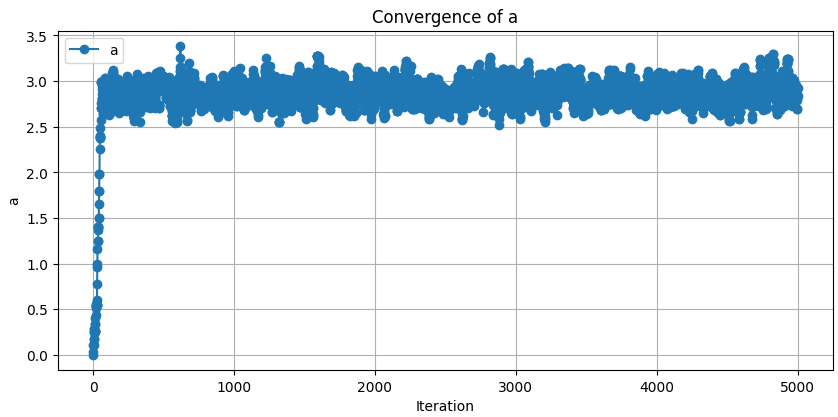
\includegraphics[width=\linewidth]{plots/output_multivar_1.png}
    \caption{Convergence of markov chains for \( a \)}
    \label{fig:my_label}
\end{figure}

\begin{figure}[htbp]
    \centering
    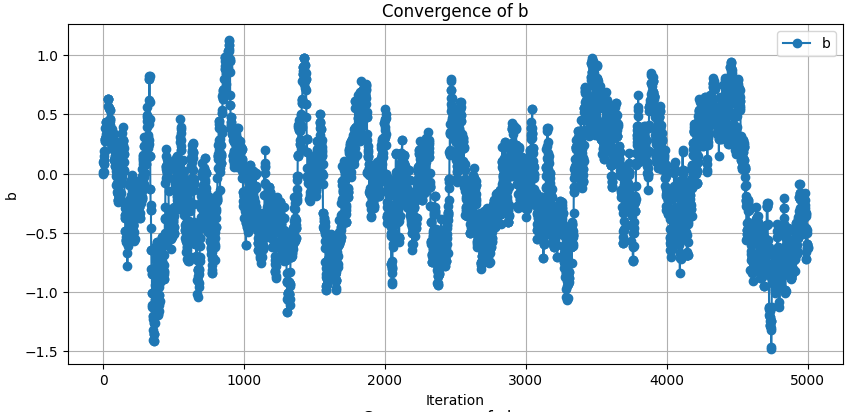
\includegraphics[width=\linewidth, height= 5cm]{plots/output_multivar_2.png}
    \caption{Convergence of markov chains for \( b \)}
    \label{fig:my_label}
\end{figure}

\begin{figure}[htbp]
    \centering
    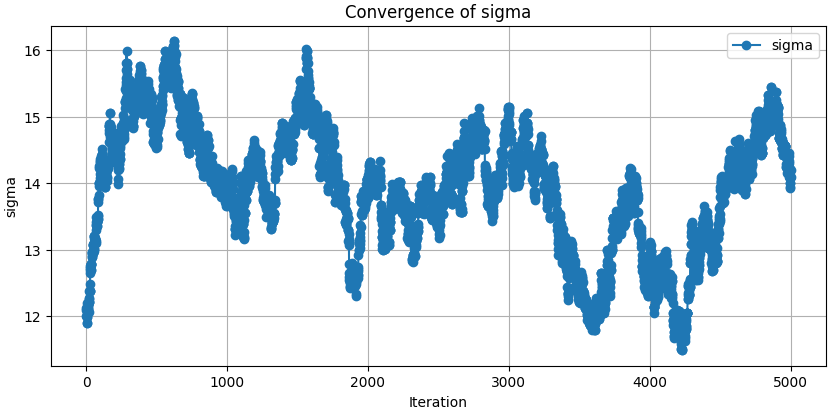
\includegraphics[width=\linewidth, height= 4cm]{plots/output_multivar_3.png}
    \caption{Convergence of metroplis chains for \(\sigma\)}
    \label{fig:my_label}
\end{figure}

\begin{figure}[htbp]
    \centering
    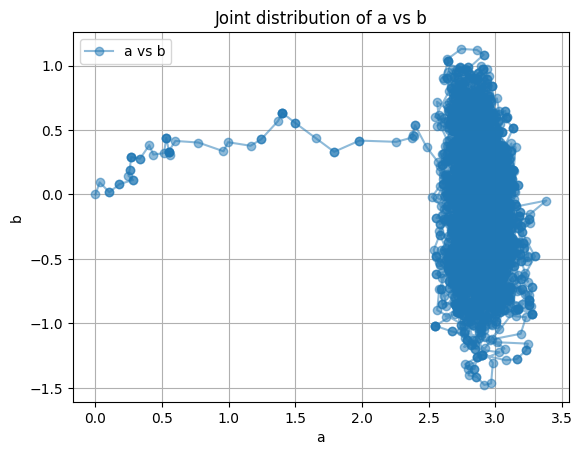
\includegraphics[width=\linewidth]{plots/output_multivar_4.png}
    \caption{Joint distribution of \(a\) and \(b\)}
    \label{fig:my_label}
\end{figure}

\begin{figure}[htbp]
    \centering
    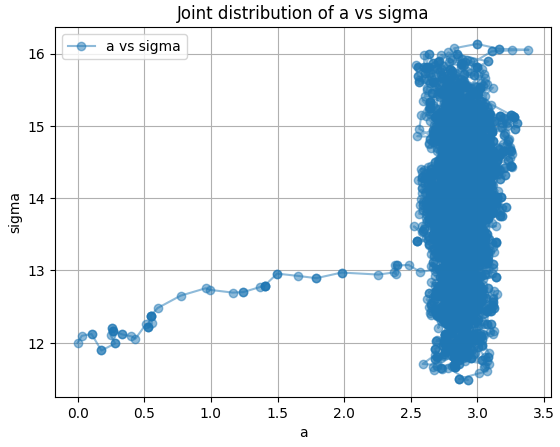
\includegraphics[width=\linewidth]{plots/output_multivar_5.png}
    \caption{Joint distribution of \(a\) and \(\sigma\)}
    \label{fig:my_label}
\end{figure}

\begin{figure}[htbp]
    \centering
    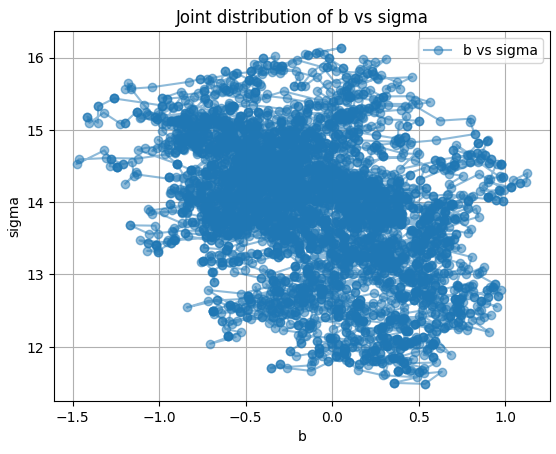
\includegraphics[width=\linewidth]{plots/output_multivar_6.png}
    \caption{Joint distribution of \(b\) and \(\sigma\)}
    \label{fig:my_label}
\end{figure}

The histogram visualization for posteriors of the parameters \( a \), \( b \), and \( \sigma \) provides insights into the probable values of these parameters given the observed data. The histograms represent the distribution of each parameter, with the x-axis denoting the parameter values and the y-axis indicating the frequency of occurrence. These visualizations offer a summary of the posterior distributions, highlighting the central tendency and variability of the parameter estimates.

\begin{figure}[htbp]
    \centering
    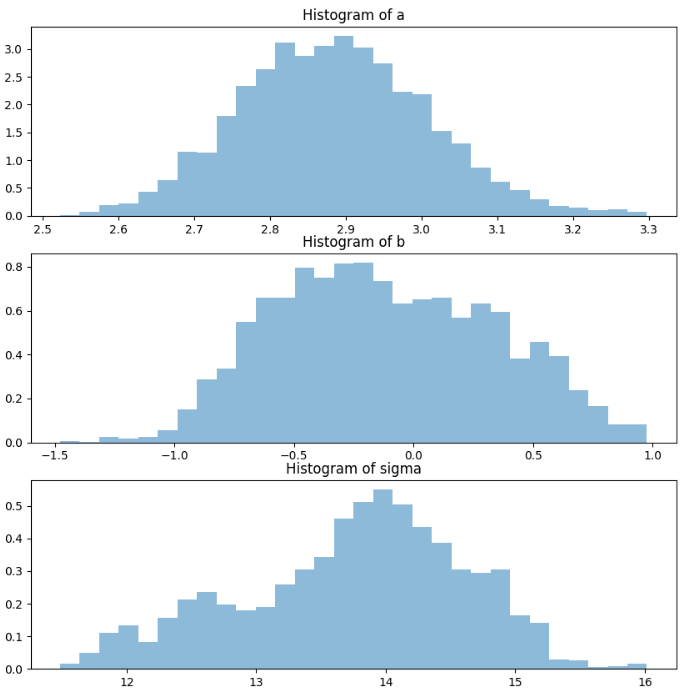
\includegraphics[width=\linewidth, height= 11cm]{plots/output_multivar_7.png}
    \caption{Histograms of the posterior distributions of \(a\), \(b\), and \(\sigma\)}
    \label{fig:my_label}
\end{figure}

\begin{figure}[htbp]
    \centering
    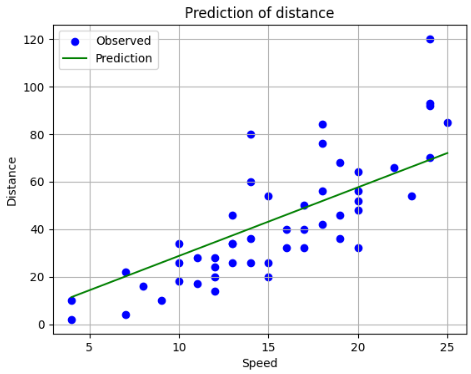
\includegraphics[width=\linewidth, height= 7cm]{plots/output_multivar_8.png}
    \caption{Prediction of stopping distances based on the linear model}
    \label{fig:my_label}
\end{figure}